\graphicspath{{images/}}

\section{\thesection~Introduction}
\label{sec:introduction}

% Expand motivation, describe QFA, discuss alternative approaches.

% Dummy \citet{Lawless2010} citations \citep{Heydari2016} \citep{Addinall2008}.


The bacteria \textit{Eschericia Coli} and yeast \textit{Saccharomyces
  cerevisae} are unicellular organisms studied as a model prokaryote
and eukaryote respectively. They grow in colonies, where cells may (be
clones originating from a single cell or) belong to different genetic
strains originating from different individual cells. In favourable
conditions, growth is exponential and this makes growth rate a major
component of fitness; faster growing strains quickly come to dominate
the population. For unicellular organisms, growth rate is equal to
cell cycle progression rate. Evolutionary pressure has led to rapidly
dividing organisms with a compact genome of essential genes. These
genes have been conserved in other species over billions of years of
evolution. The eukaryote \textit{S. cerevisae}, is particularly useful
for the study of other eukaryotes such as humans.

The growth rate of microbial organisms is measurable and is often used
to determine fitness. In experiments, cell cultures are commonly grown
in two types of medium. In spot atests (phenotypic array), cultures are pinned or
inoculated onto the surface of a solid agar containing nutrients. In
liquid culture assays, cultures are mixed in a liquid medium
containing nutrients. In both cases cultures are incubated and growth
is observed. Identical strains grow differently between the two
mediums and disagreement between fitness estimates is currently an
issue. I did not focus on this issue and used data exclusively from
experiments using solid agar.




The bacteria \textit{Eschericia Coli} and yeast \textit{Saccharomyces
  cerevisae} are unicellular organisms studied as a model prokaryote
and eukaryote respectively. They grow in colonies, where cells may (be
clones originating from a single cell or) belong to different genetic
strains originating from different individual cells. In favourable
conditions, growth is exponential and this makes growth rate a major
component of fitness; faster growing strains quickly come to dominate
the population. Growth rate is measurable and is often used to
determine the fitness of microbial organisms. For unicellular
organisms, growth rate is equal to cell cycle progression
rate. Evolutionary pressure has led to rapidly dividing organisms with
a compact genome of essential genes. These genes have been conserved
in other species over billions of years of evolution. The eukaryote
\textit{S. cerevisae}, is particularly useful for the study of other
eukaryotes such as humans.




% Where do cells grow surfaces films.

\subsection{\thesubsection~Subsection}

\begin{Figure}
  \centering
  \includegraphics[width=\linewidth]{p15_section/p15_section}
  \captionof{figure}{\textbf{4x5 section of a QFA plate.} Taken from a
    16x24 format solid agar plate inoculated with dilute
    \textit{S. cerevisae} cultures.
  Image captured at \(\sim\)2.5d after inoculation and incubation at
  27\(^{\circ}C\).}
  \label{fig:p15_section}
\end{Figure}


\begin{Figure}
  \centering
  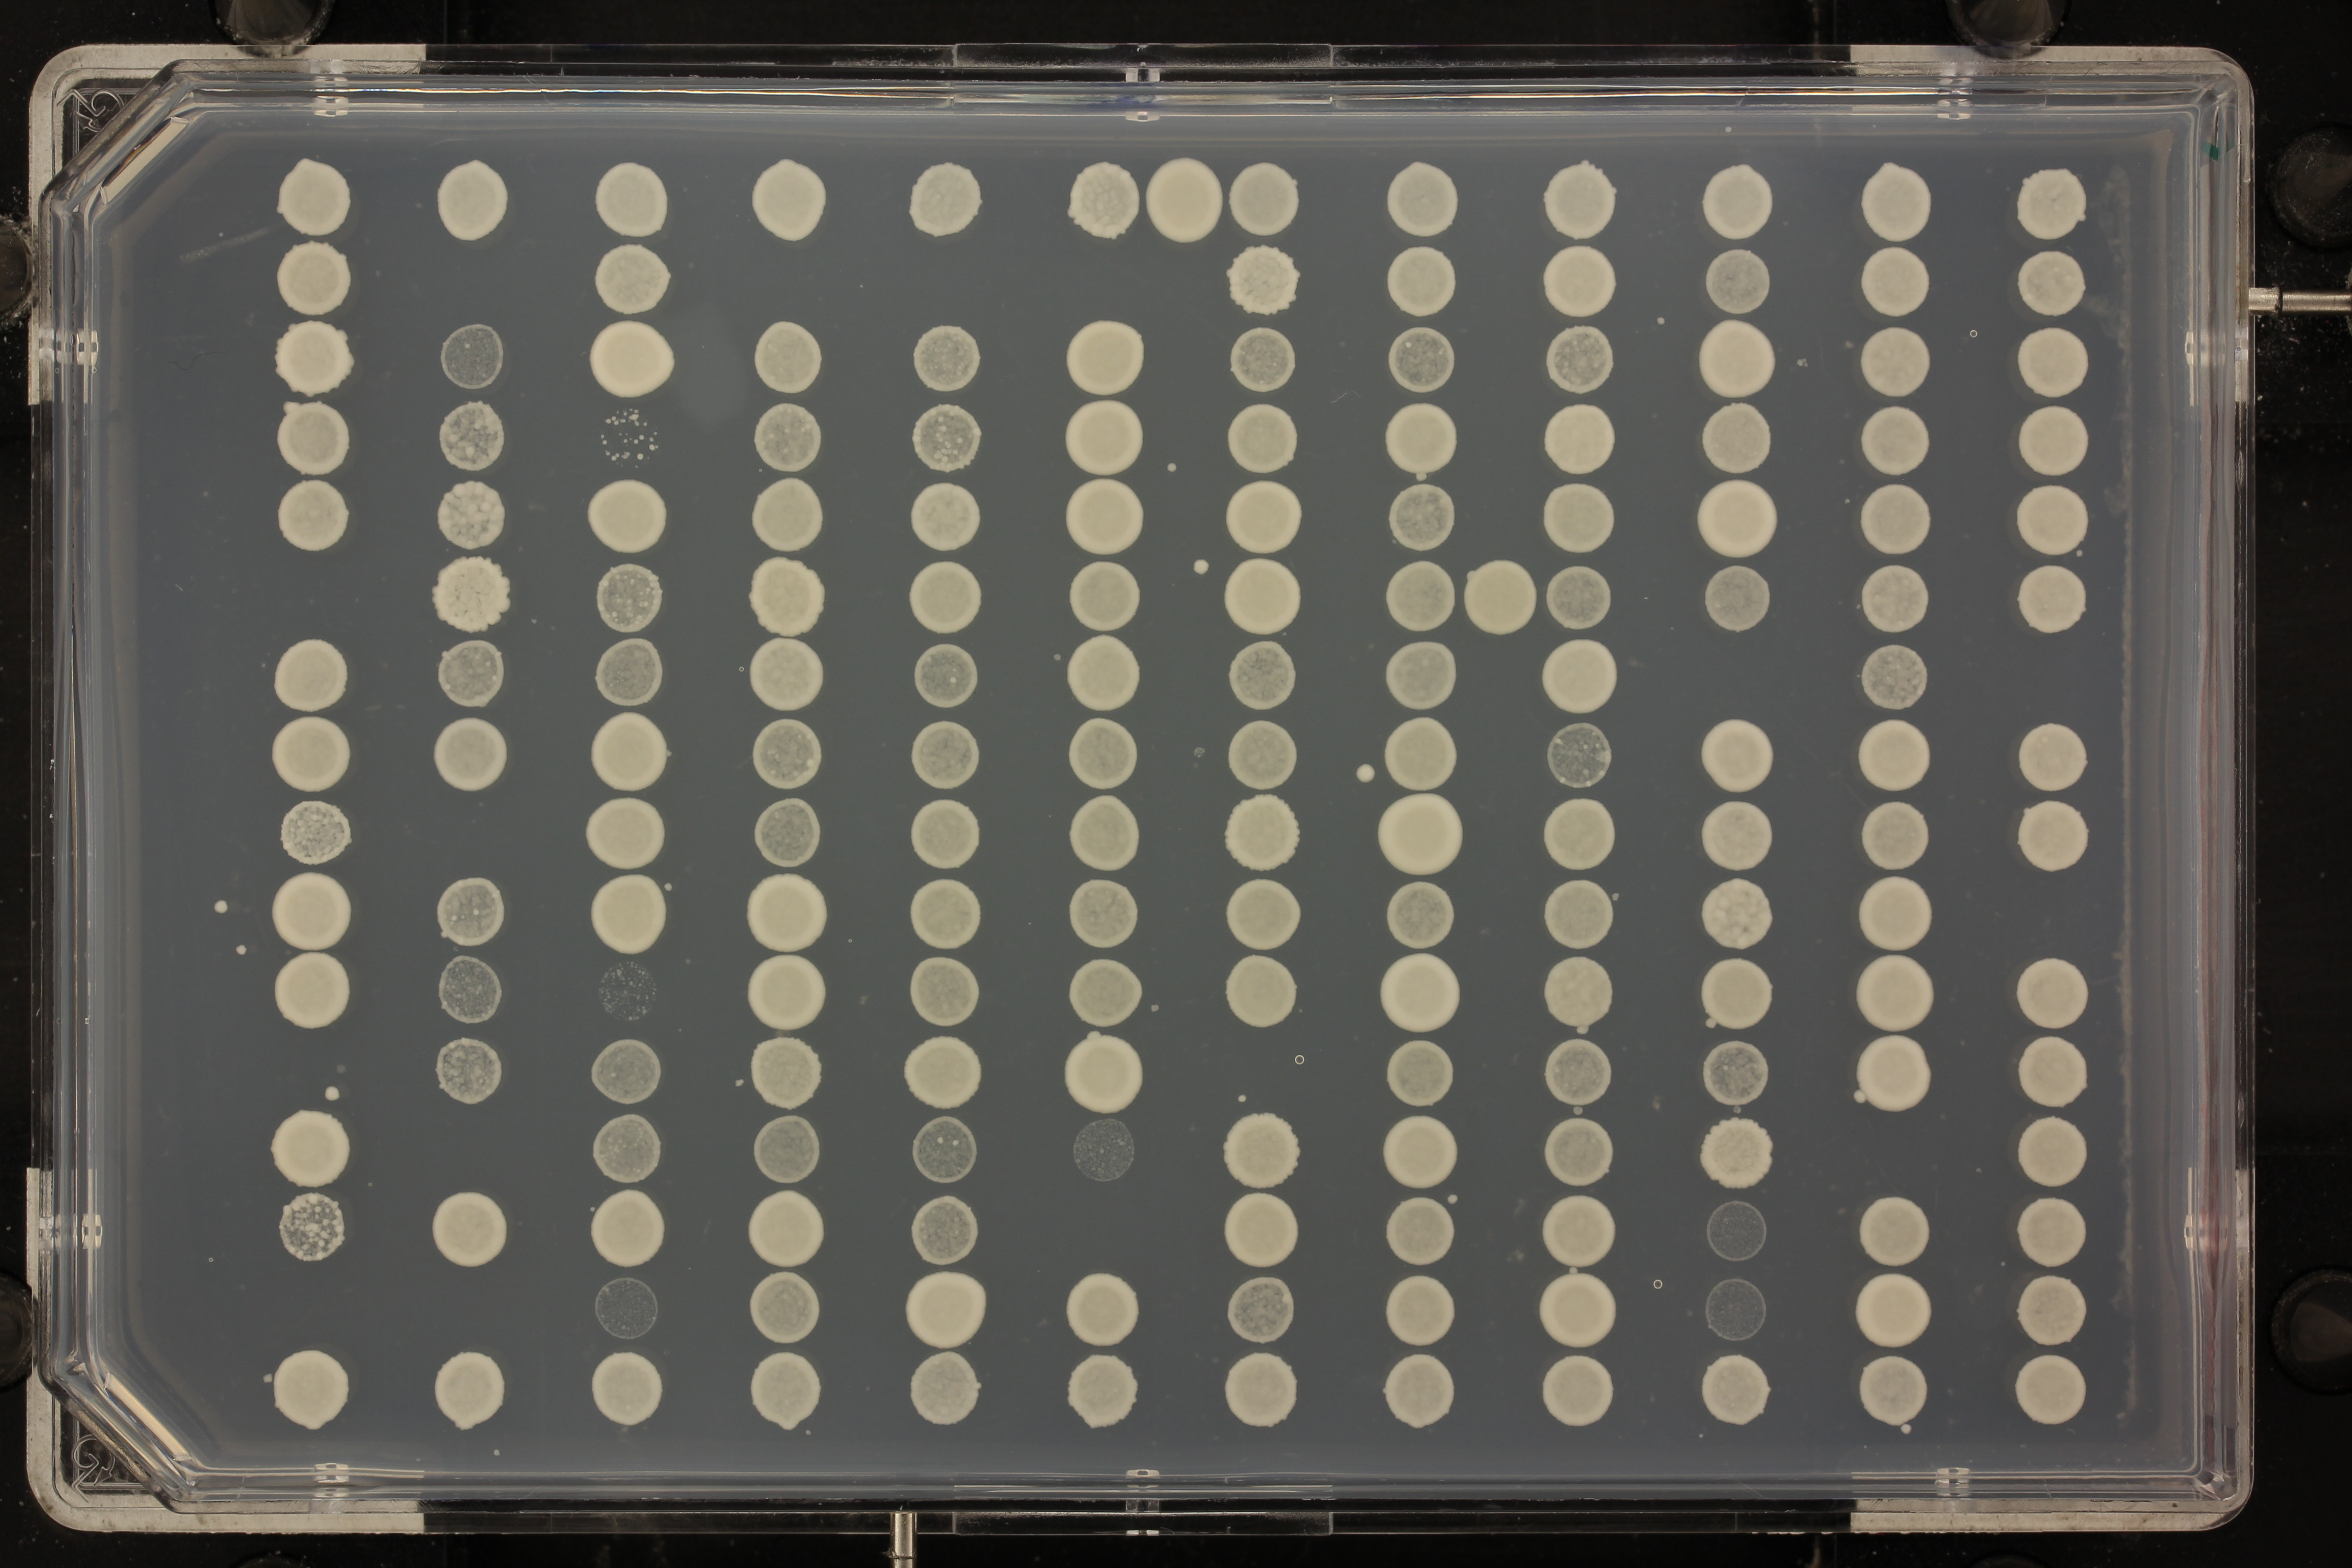
\includegraphics[width=\linewidth]{stripes/final/striped}
  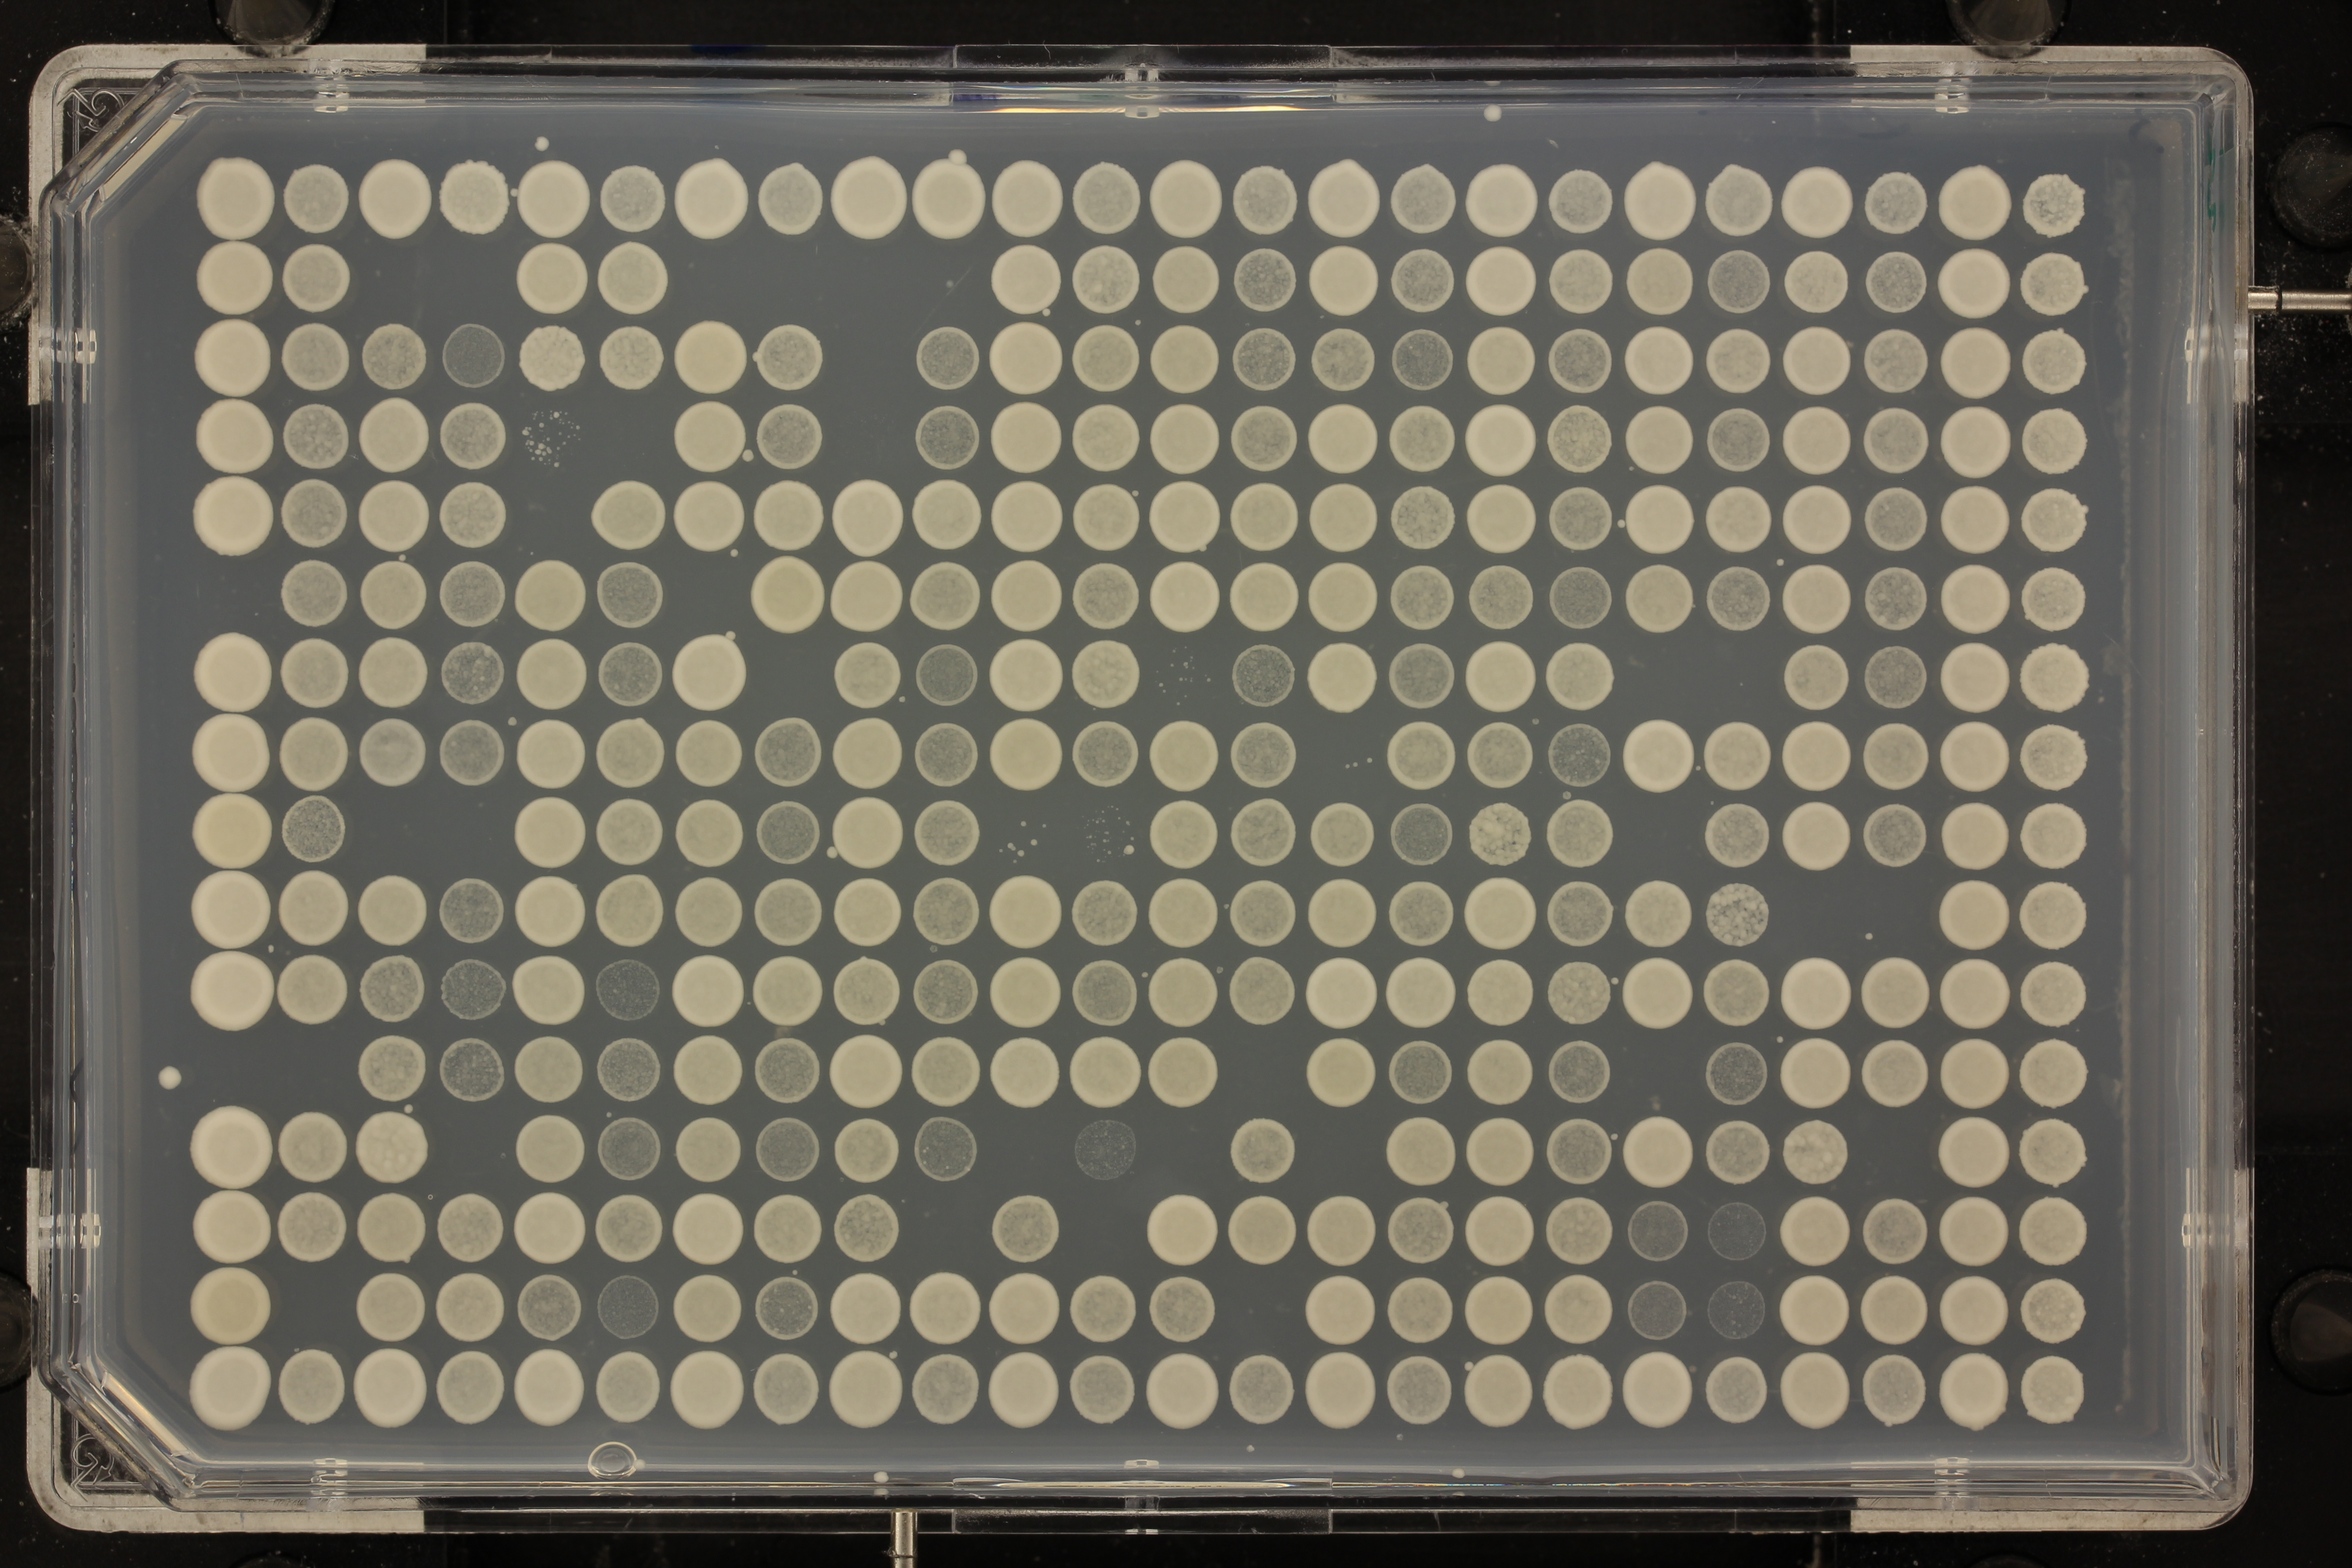
\includegraphics[width=\linewidth]{stripes/final/filled}
  \captionof{figure}{\textbf{An experiment designed to examine
      competition.}\\
    A) QFA plate inocluated with a more concentrated
    \textit{S. Cerevisae} inoculum (no cells inocluated on alternative
    columns).\\
    B) Same as in A, but with strains of similar growth rate
    inoculated in the positions missing in A.}
  \label{fig:stripes_images}
\end{Figure}



%%% Local Variables:
%%% mode: latex
%%% TeX-master: "report"
%%% End:
